%!TEX root = ../../../adrien_gomar_phd.tex

In Section~\ref{sec:sm_hb_multi}, the multi-frequential harmonic
balance approach has been presented. In this method,
the frequencies can be chosen arbitrarily. This becomes particularly
interesting when dealing with signal/ flow field composed of segregated
frequencies. For instance, let us consider the linear advection toy problem
as defined in Sec.~\ref{sec:toy_convection} with 
a perturbation 
in the form of a sum of two sine functions,
applied at the left boundary:
\begin{equation}
    u_l(t) = \sin(\omega t) + \sin(22 \omega t).
    \label{eq:multifreq_inj_func}
\end{equation}

\subsection{Using a mono-frequential approach}

Obviously, computing the advection of such a signal using
a classical time-marching scheme would require to discretize the
smaller period. The largest frequency
(here $f_2 = 22$~Hz) acts as a bottleneck as the time-step will be chosen
according to this frequency. The cost of the time-marching
scheme scales with the ratio of $f_1= 1 $~Hz and $f_2=22$~Hz. This
means that compared to a computation where only $f_1$ or only $f_2$
is involved, the cost will be multiplied by~22.

This olds true when computing the solution with the mono-frequential
harmonic balance approach. The frequencies can not be chosen arbitrarily.
Therefore, to compute such a configuration, a $N=22$ harmonic computation
will be needed to be spectral accurate. To emphasize that, mono-frequential
HB computations are run with 1 to 25~harmonics.
As made in the previous Section~\ref{sec:sum_sine}, 
for six chosen computations of the~25 computations, 
we show spatial distributions of the solution
at three time instances, namely, $t=0$, $t=T/3$ and $t=2T/3$.
It is shown in Fig.~\ref{fig:inj_multifreq_tsm}.
\begin{figure}[htb]
  \centering
  \subfigure[$N=1$]{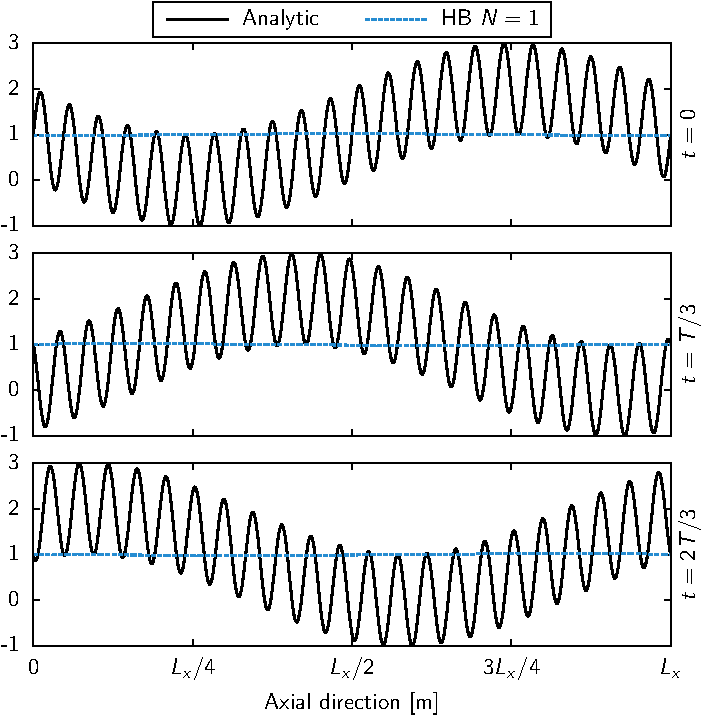
\includegraphics[width=.35\textwidth]{convection_multifreq_tsm_N1.pdf}}
  \subfigure[$N=5$]{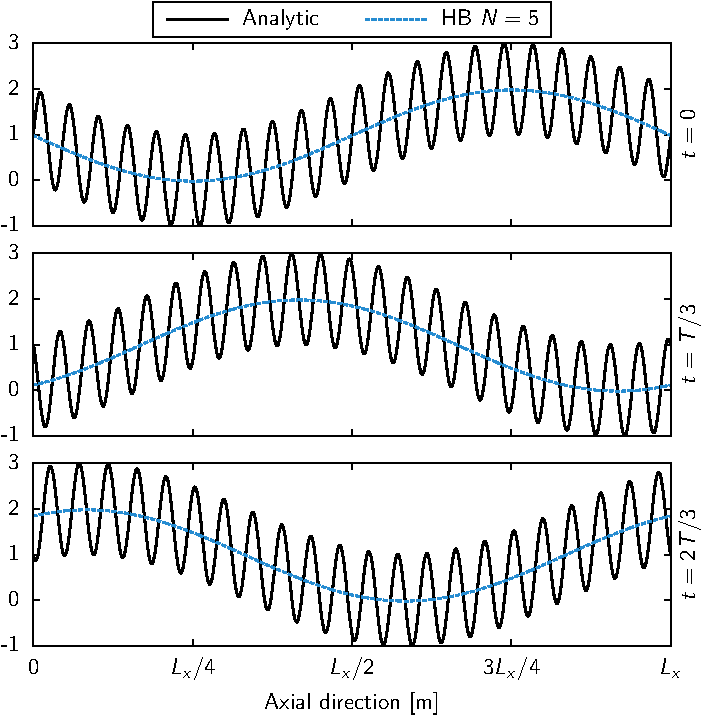
\includegraphics[width=.35\textwidth]{convection_multifreq_tsm_N5.pdf}}
  \subfigure[$N=11$]{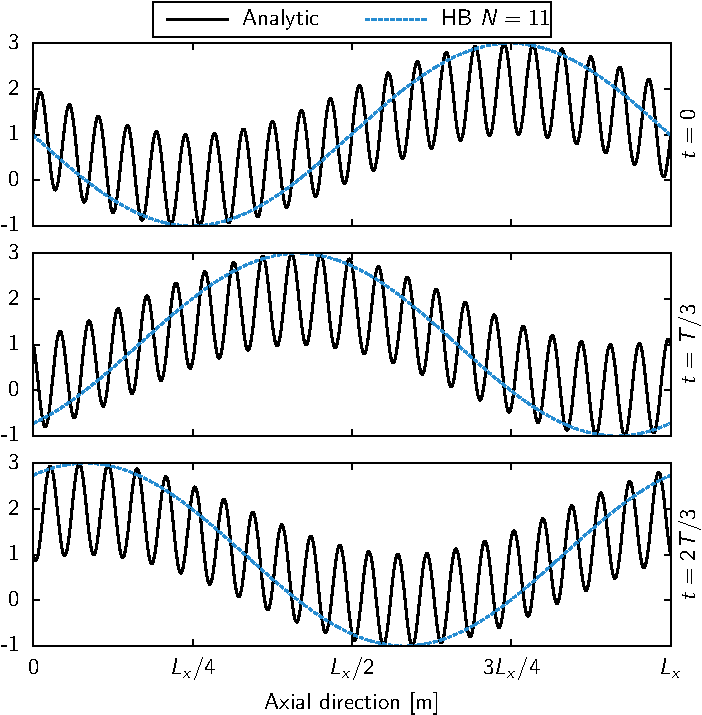
\includegraphics[width=.35\textwidth]{convection_multifreq_tsm_N11.pdf}}
  \subfigure[$N=16$]{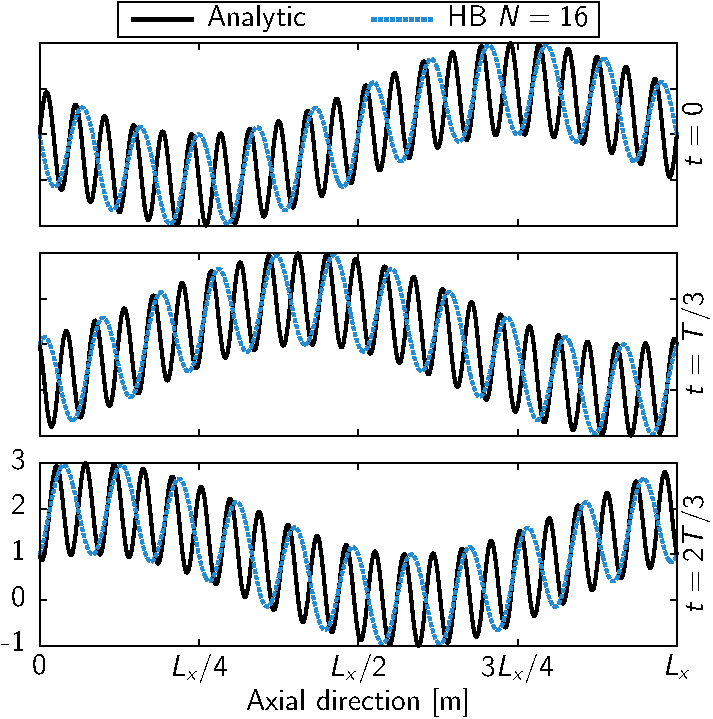
\includegraphics[width=.35\textwidth]{convection_multifreq_tsm_N16.pdf}}
  \subfigure[$N=22$]{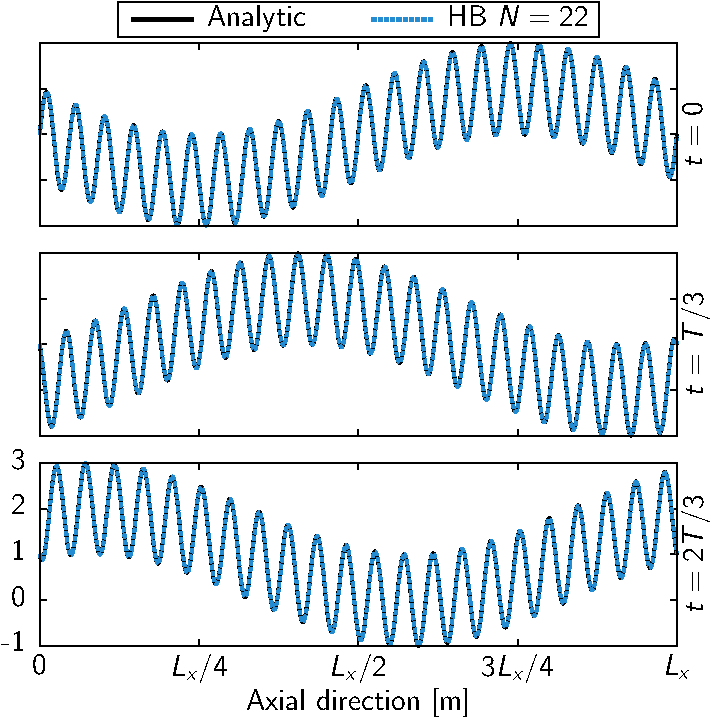
\includegraphics[width=.35\textwidth]{convection_multifreq_tsm_N22.pdf}}
  \subfigure[$N=23$]{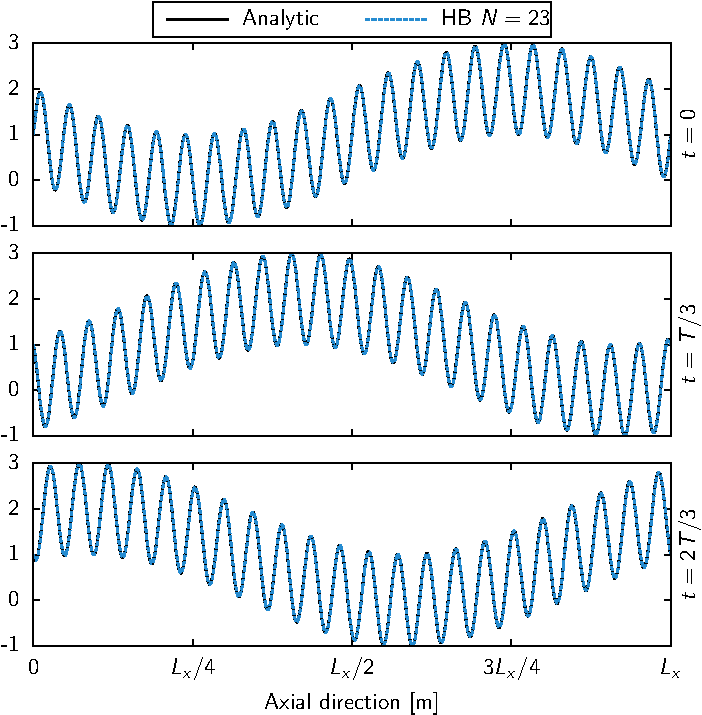
\includegraphics[width=.35\textwidth]{convection_multifreq_tsm_N23.pdf}}
  \caption{Linear advection of a sum of two segregated sine functions: 
  numerical solutions at different time instances for different numbers of harmonics.}
  \label{fig:inj_multifreq_tsm}
\end{figure}
Again, the accuracy in capturing the injected function
improves with the number of harmonics,
until it reaches the frequency content
of the injected signal, i.e. 22~harmonics.
After that, the results of the HB computations are
superimposed with the analytical solution. 
The problem is that with such a separation of frequencies,
the mono-frequential version suffers from the same
problems as a classical time-marching scheme.

To quantitatively analyze the results,
the discrete $\mathcal{L}_2$-norm of the error 
in time is computed over all the time instances
at each grid points over the domain.
Then, the average in space is computed.
It is shown in Fig.~\ref{fig:conv_multifreq_tsm} for the
mono-frequential HB computations ranging from one to~25
harmonics.
\begin{figure}[htb]
  \centering
  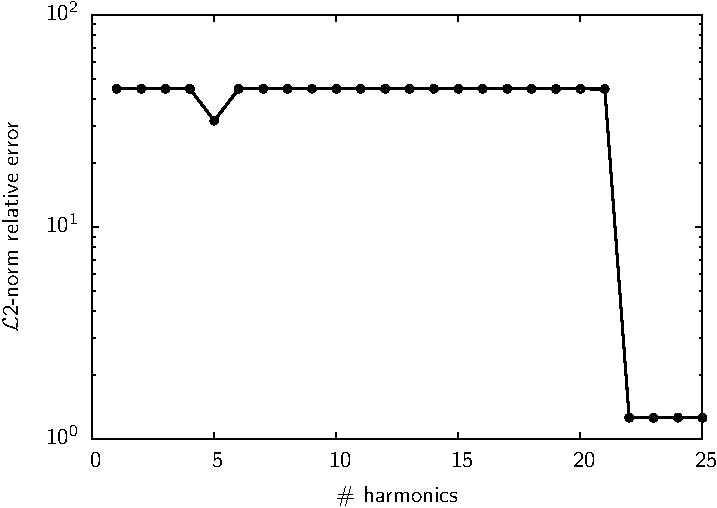
\includegraphics[width=.5\textwidth]{convection_multifreq_error.pdf}
  \caption{Linear advection of a sum of two segregated sine functions: convergence of the mono-frequential HB method error.}
  \label{fig:conv_multifreq_tsm}
\end{figure}
When the number of harmonics
used to compute the solution is higher than the content of the spectrum,
then the error decreases drastically. The spectral accuracy is retrieved
but only starting at $N=22$.
In fact, similar as in Sec.~\ref{sec:sum_sine},
the injected function is indefinitely differential and periodic
leading an infinite convergence slope. We can observe a slight local convergence
for the $N=5$ harmonics HB computation. This is due to the fortunate 
capture of the low-frequency pattern of the injected function.

\subsection{Using a multi-frequential approach}

One of the advantage of the multi-frequential HB method introduced in Sec.~\ref{sec:sm_hb_multi}
and used in this thesis is that it can take arbitrary frequencies into account.
In the case of an injected signal with a large frequency separation, the
benefit might be tremendous. Let us consider again the signal defined in 
Eq.~\eqref{eq:multifreq_inj_func} and compute one HB simulation using 
$f_1=1$~Hz and $f_2=22$~Hz as input frequencies. This gives a $N=2$
computation that is nine times faster than the $N=22$ converged mono-frequential
HB computation.
Again
we show spatial distributions of the solution
at three time instances, namely, $t=0$, $t=T/3$ and $t=2T/3$
in Fig.~\ref{fig:inj_multifreq_hb}.
\begin{figure}[htb]
  \centering
  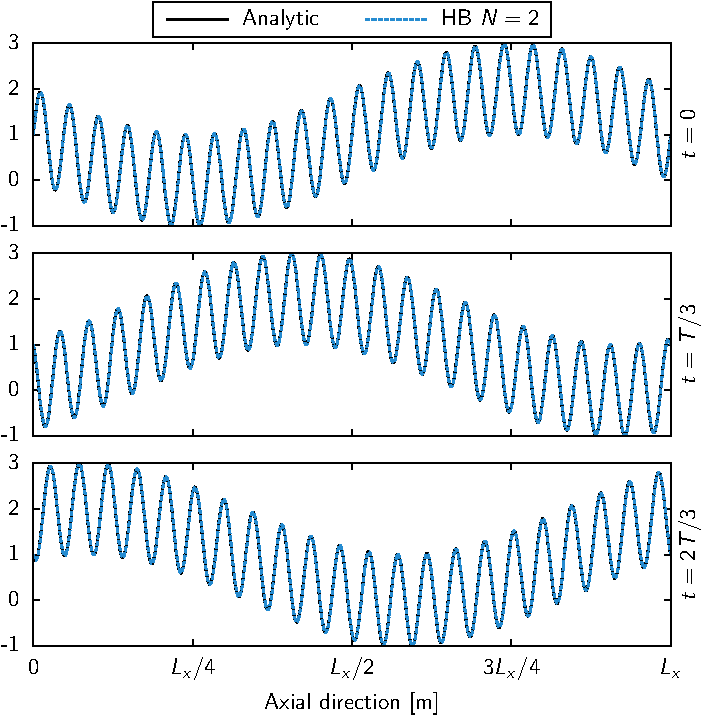
\includegraphics[width=.35\textwidth]{convection_multifreq_hbt_N2.pdf}
  \caption{Linear advection of a sum of two segregated sine functions: 
  numerical solutions at different time instances for different numbers of harmonics using the
  multi-frequential harmonic balance method.}
  \label{fig:inj_multifreq_hb}
\end{figure}
With only two input frequencies, the multi-frequential
HB solution is superimposed with the analytical solution.
Moreover, the $\mathcal{L}2$-norm of the error is 
exactly the same as the one of the $N=22$ mono-frequential
approach.


\subsection{Toward aeroelasticity of contra-rotating open rotors}
The reason why we studied the multi-frequential harmonic balance
approach for the aeroelasticity of contra-rotating open rotors
is that it is a problem where the major frequencies are most
likely to be segregated as shown previously in Chap.~\ref{cha:cror} and
Chap.~\ref{cha:ael}. In this framework, the multi-frequential
harmonic balance approach looks very promising according to the results
seen in this Chapter.
